\documentclass[a4paper, 10pt, conference]{IEEEtran} % Use this line for a4 paper

\usepackage{graphics} % for pdf, bitmapped graphics files
\usepackage{epsfig} % for postscript graphics files
\usepackage{mathptmx} % assumes new font selection scheme installed
\usepackage{times} % assumes new font selection scheme installed
\usepackage{amsmath} % assumes amsmath package installed
\usepackage{amssymb}  % assumes amsmath package installed

% Custom packages
\usepackage{algorithm}
\usepackage{algpseudocode} % pour avoir l'environnement algorithmic

\title{\LARGE \bf
--- Electronical Engineering Note --- \\
Engineering of a 94kHz 15A sensorless quadricopter ESC
}

\author{Stepane Binon and Guilhem Andrieu% <-this % stops a space
	\thanks{Bare Metal Foundry}
	\thanks{\tt\small stepane.binon@gmail.com}
}

\begin{document}

\maketitle
\thispagestyle{empty}
\pagestyle{empty}

%%%%%%%%%%%%%%%%%%%%%%%%%%%%%%%%%%%%%%%%%%%%%%%%%%%%%%%%%%%%%%%%%%%%%%%%%%%%%%%%
\begin{abstract}
To come
\end{abstract}


%%%%%%%%%%%%%%%%%%%%%%%%%%%%%%%%%%%%%%%%%%%%%%%%%%%%%%%%%%%%%%%%%%%%%%%%%%%%%%%%
\section{Introduction}

The goal of this document is to sumarize the though process, the choices and calculations made during the design of an ESC aimed at being used in an autonomous race quadricopter. 

This project is part of the Bare Metal Foundry, an association which aims at having serious fun with engineering challenges and is also our first attemps at PCB design, both as engineers and association. In this context, the Kururugi-ESC has a central place as a vector of learing and as one of the most important part of a quadricopter, the ESC being the deepest loop of control, the fastest, and thus the deadliest in case of crash. 

We wanted to do this design from scratch to, in addition of learning, gain complete control of the hardware (h/w) and matching the performances we needed. Hence, for now, we do not aim to make it compatible with any ESC software existing as we will develop a custom one in C++, this will be the subject of an article to come. For Version 1.0 of this project, it is aimed to contribute in the following points:
\begin{itemize}
    \item The production of a 24 to 64kHz, 15A continuous, 95\%D (Duty Cycle), 4S to 6S, and sensorless ESC that can work both with Six-Step Control (SSC) and Field-Oriented Control (FOC). The caracteristic are presented in detail in Figure X;
    \item The presentation of measure and results obtained;
    \item A complete guideline on how to design a such an ESC PCB, that we hope is state of the art.
\end{itemize}

\begin{figure}[h] % placement: top of page
    \centering
    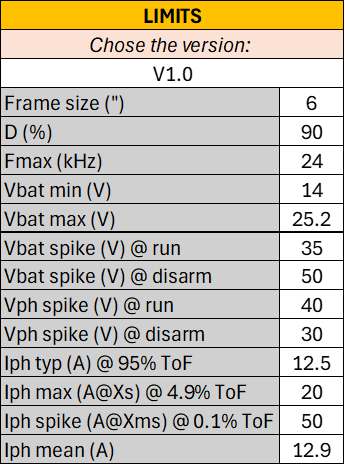
\includegraphics[width=0.45\columnwidth]{figures/limits.png}
    \caption{Limits}
    \label{fig:limits}
\end{figure}


The Version 1.0 of the Kururugi-ESC will be oriented toward getting it working whereas next versions goals are aimed toward research. One particular point we are interested in is to have the SSC working on a 128kHz PWM, which would bring challenges both for the electronical and coding aspects.

The rest of this paper is organized as follows. Section II will be about the schmatics and selection of components. Section III will present the layout. Section II will exposes results


%%%%%%%%%%%%%%%%%%%%%%%%%%%%%%%%%%%%%%%%%%%%%%%%%%%%%%%%%%%%%%%%%%%%%%%%%%%%%%%%
\section{Schematic and choice of components}

An ESC is composed of N main sectionsparts
\begin{itemize}
    \item An MCU (Micro Controller Unit), responsible for the overall control of the behaviour, mainly communication with the Flight Controller (FC) and control of the power section behaviour;
    \item Analog to Digital Converters (ADC) and Operational Amplificator (OpAmp), which are used to translate analog signal as tension and current on each phase to the digital language of the MCU. As space is constrained on this PCB, the MCU internal ADC and OpAmp will be used;
    \item The power section, composed of the 3 half bridge needed to control the Brushless Direct Current Motor (BLDC), get the necessary analog outputs for the MCU and also power the ICs present on the PCB. This is from far the most complexe part of an ADC as it require fine control over very important electron flows;
\end{itemize}

\subsection{Half-Bridge Design}

A BLDC motor is driven by electronically commutating three phases using three half-bridges. The primary function of the ESC is to ensure correct commutation to maintain rotation. Its secondary function is to regulate motor speed via PWM control.

The half-bridge stage is the most critical part of the ESC, as it forms the interface between the power domain, where high battery and motor currents flow; the gate-drive domain, responsible for controlling the MOSFET switching transitions; and the logic and sensing domain, where low-level control and measurement signals must remain accurate despite the presence of high dV/dt and dI/dt switching events.

The main design challenges are:
\paragraph{Power integrity}
The stage must conduct high battery currents with minimal losses while remaining thermally stable. This includes proper MOSFET selection, controlled switching transitions, and adequate heat dissipation.

\paragraph{Signal integrity}
Accurate voltage and current sensing is required for sensorless FOC. High dV/dt and dI/dt switching must not corrupt low-level measurement signals. Gate nodes must remain immune to parasitic coupling to prevent false triggering.

\paragraph{Switching integrity}
The MOSFETs must be driven quickly and predictably. The gate capacitance must be charged and discharged with sufficient current to minimize time spent in the linear region. Shoot-through must be prevented through proper dead-time control. The bootstrap capacitor and gate driver must sustain the required charge over all operating conditions. \\

\subsubsection*{MOSFET Selection}

Beyond maximum current rating at elevated temperature, MOSFET selection is primarily driven by total gate charge $Q_g$ and on-resistance $R_{DS,on}$. The gate charge defines the energy required for each switching event: a higher $Q_g$ increases switching losses and slows transitions. The on-resistance determines conduction losses while the device is fully enhanced. At low PWM frequency, conduction losses dominate; as switching frequency increases, switching losses become predominant.

Conduction losses per MOSFET are approximated by
\[
P_{cond} = R_{DS,on} \cdot I^2 \cdot D
\]
and switching losses by
\[
P_{sw} = V \cdot I \cdot (t_{rise} + t_{fall}) \cdot f_{sw}.
\]

For Kururugi-ESC-V1.0, six Texas Instruments CSD18540Q5B MOSFETs are selected, with $Q_g = 41\,\text{nC}$ and $R_{DS,on} = 2.2\,\text{m}\Omega$. These devices provide a competitive compromise between conduction and switching performance and are readily available from JLCPCB. Estimated losses are $P_{\text{loss,mean}} = 0.48\,\text{W}$ and $P_{\text{loss,max}} = 1.02\,\text{W}$. A 10\,V gate drive is used to ensure low $R_{DS,on}$ and stable switching behavior. \\


\subsubsection*{Gate Driver Design}

The Infineon 2EDL8024 is selected as gate driver due to its high peak drive capability (3\,A source, 4–5\,A sink) and compact footprint. A 10\,V gate-drive voltage is used to ensure full MOSFET enhancement while maintaining margin against UVLO.

\paragraph{Bootstrap capacitor sizing}

The high-side supply relies on a bootstrap capacitor. Its dimensioning must guarantee sufficient charge to fully drive the MOSFET during the maximum on-time without triggering UVLO.

The maximum allowable bootstrap voltage drop is
\[
\Delta V_{boot,max} = V_{DD} - V_F - V_{HBR} - V_{HBH} = 3.22\,\text{V}.
\]

The total charge required during one switching cycle includes the MOSFET gate charge and driver-related consumption:
\[
Q_{BS} = Q_g + \frac{I_{HB} + (I_{HBS} + I_{pulldown}) D_{max}}{F_{sw}} = 155\,\text{nC}.
\]

\[
I_{pulldown} = V_{boot,max} / R_{pulldown}
\]

\[
C_{boot} = \frac{C_{boot,min}}{1-{k_{derating}}}*S_{C_{boot}}
\]

\[
t_{recharge} = \frac{1-D}{F_{SW}} - t_{blank@V_{SW}=0}
\]

\[
V_{boot,min} = V_{DD}-\Delta V_{boot,max}
\]

\[
V_{boot,max} = V_{DD}-V_f
\]

\[
V_{boot@D_{max}} = V_{boot,max}*(1-e^{-\frac{t_{recharge}}{R_{boot,ext}*C_{boot}}})
\]

\[
V_{boot,max @ D_{max}} = V_{\text{boot,max}} - y\left(V_{\text{boot,max}} - V_{\text{boot,min}}\right)
e^{-\frac{t_{\text{recharge}}}{R_{\text{eq}}C_{\text{boot}}}}
\]

\[
R_{eq} = \frac{  R_{boot,ext} * R_{boot,int}   }{    R_{boot,ext} + R_{boot,int} }
\]

\[
R_{eq,on} = \frac{R_{pu,hs}+R_{pu,ls}}{2} + R_{g,on+off}
\]

\[
R_{eq,off} = \frac{R_{pd,hs}+R_{pd,ls}}{2} + R_{g,eq,off}
\]

\[
I_{max,on} = V_{boot,max} / R_{eq,on}
\]

\[
I_{max,off} = V_{boot,max} / R_{eq,off}
\]

\[
R_{GD,mean} = \frac{D_{max}*(R_{pu,hs}+R_{pu,ls}) +(1-D_{max})*(R_{pd,hs}+R_{pd,ls})}{4}
\]

\[
R_{g,mean} = \frac{D_{max}*R_{g,on+off} +(1-D_{max})*R_{g,eq,off}}{2}
\]

\[
P_{Rg,mean} = \frac{R_{g,mean}}{R_{g,mean}+R_{GD,mean}}*P_{g,loss}
\]

\[
P_{R_{GD},mean} = P_{g,loss}-P_{Rg,mean}
\]

\[
R_{g,eq,off} = \frac{   R_{g,on+off} * R_{g,on+off}   }{   R_{g,on+off} + R_{g,on+off}  }
\]

\[
P_{g,loss} = P_{g,loss,min}*S
\]

\[
P_{g,loss,min} = Q_g * V_{boot,max} * F_{SW}
\]

The minimum bootstrap capacitance is therefore
\[
C_{boot,min} \ge \frac{Q_{BS}}{\Delta V_{boot,max}} = 48\,\text{nF}.
\]

Applying a 40\% DC-bias derating and a safety factor of 2 leads to a selected value of 160\,nF. The resulting bootstrap time constant is $\tau_{boot} = 0.66\,\mu\text{s}$, ensuring recharge within the available low-side conduction window. The expected bootstrap voltage evolves from $V_{boot0}=8.45\,\text{V}$ to $V_{boot,final}=9.29\,\text{V}$, converging toward $9.49\,\text{V}$.

\paragraph{Gate resistors and switching behavior}

Gate resistors are selected to shape switching speed and control EMI. The chosen values are $R_{g,on+off}=5.1\,\Omega$ and $R_{g,off}=10\,\Omega$, with a 10\,k$\Omega$ gate pulldown resistor. The effective driver resistance results in peak gate currents of
\[
I_{on,max} = 1.56\,\text{A}, \qquad
I_{off,max} = 2.50\,\text{A}.
\]

The corresponding gate charge time constant is $\tau_{Qg,on}=976\,\text{ns}$. These resistors values are intentionally conservative for initial validation to limit EMI while maintaining acceptable switching losses. It should be possible to get much faster switching.

\paragraph{Loss distribution}

Per MOSFET, conduction losses are estimated at 0.19\,W. Gate-drive related dissipation is distributed as 0.03\,W inside the driver IC, 0.107\,W in the combined turn-on/off resistor, and 0.05\,W in the turn-off resistor. Maximum conduction losses per ESC are estimated at 0.38\,W.

This configuration provides controlled switching dynamics, sufficient bootstrap stability, and predictable thermal behavior across operating conditions. The balance in power dissipation should permit the use of small package resistors.





%\subsubsection*{Gate Driver Design}
%
%The Infineon 2EDL8024 gate driver is selected for its high peak source and sink currents (3\,A pull-up and 4–5\,A pull-down) in a compact package. Its role is to charge and discharge the MOSFET gate rapidly, thereby minimizing switching losses, reducing time spent in the linear region, and ensuring predictable and robust switching under all operating conditions with minimized EMI.
%
%It is supported by a boost capacitor, which must be sized to ensure that the MOSFET can be fully filled even at high duty cyle. To compute it, we first compute the maximum tolerable voltage difference before UVLO is triggered.
%$\Delta V_{Cboot\_max} = V_{dd} - V_F - V_{HBR} - V_{HBH} = 3.2V$
%
%Then, a capacitance can be computed taking into account the gate capacitace and the leakage during the high time of the mosfet, as given bellow  $Q_T = Q_g + \frac{I_{HB}+(I_{HBS}+I_{pulldown})*D_{max}}{F_{SW}} = 155nC$
%
%Finally, Cboot_min is computed using $C_{boot\_min} \geq \frac{Q_T}{V_{Cboot\_max}} =48nF$ taking into account a DC derating of 40% and a 2 safety maring, we will chose a 160nF capacitor.
%
%Finnaly, we chose Rg,on and Rg,off to be respectively 5.1kOhm and 10kOmh, for a Ion=1.56A and Ioff=2.50A, these value are kept low on purpose to ensure low EMI on first test. 








